% !TeX spellcheck = en_US
% !TeX program = pdflatex

\documentclass{beamer}
\usepackage[utf8]{inputenc} % russian, do not change
\usepackage[T2A, T1]{fontenc} % russian, do not change
\usepackage[english, russian]{babel} % russian, do not change

% fonts
%\usepackage{fontspec} % different fonts
%\setmainfont{Times New Roman}
\usepackage{setspace,amsmath}
\usepackage{amssymb} %common math symbols
\usepackage{dsfont}

% utilities
\usepackage{systeme} % systems of equations
\usepackage{mathtools} % xRightarrow, xrightleftharpoons, etc
\usepackage{array} % utils for tables
\usepackage{makecell} % multirow for tables
\usepackage{subfiles}
\usepackage{hyperref}
\hypersetup{pdfstartview=FitH,  linkcolor=blue, urlcolor=blue, colorlinks=true}
\usepackage{framed} % advanced frames, boxes
\usepackage{graphicx}
\usepackage{caption}
\usepackage{subcaption} % captions for subfigures
\usepackage{color}
\usepackage{chngcntr} % change counters
%\counterwithout*{section}{chapter} % continue sections enumeration with chngcntr


% styling
\usetheme{default}
\usepackage{float} % force pictures position
\floatstyle{plaintop} % force caption on top
\usepackage{enumitem} % itemize and enumerate with [noitemsep]
\setlength{\parindent}{0pt} % no indents!

% misc
\graphicspath{{./img/}}
\newcommand{\myPictWidth}{.95\textwidth}
\newcommand{\phm}{\phantom{-}}

\title{Кинетическая коррекция: Новый механизм уменьшения числа ошибок в биосинтетических процессах, требующих высокой специфичности}
\subtitle{(Kinetic Proofreading <...> [Hopfield, 1974])}
\author{Валерий Зуев}
\begin{document}
\begin{frame}[plain]
    \maketitle
\end{frame}
% \begin{frame}{Интуитивные соображения}
% \end{frame}
\begin{frame}{Big Picture}
Специфичность при чтении ДНК (и других реакциях биосинтеза) может быть увеличена по сравнению со специфичностью, обусловленной разницей средних кинетических барьеров, с помощью процесса \emph{кинетической коррекции}.

В статье описан простой кинетический путь, приводящий к такой коррекции, когда реакция сильно, но неспецифично катализируется, например, гидролизом фосфата.

Известные реакции, кажущиеся излишними, оказываются важными для осуществления коррекции.

\end{frame}

\begin{frame}{Малое число ошибок при синтезе}

Доля ошибок в простой модели синтеза:
\[ p_{err}^{(1)} = \exp \left( - \frac{\Delta G_{CD}}{RT} \right) \]

Модель с коррекцией (точность коррекции та же, что и специфичность при синтезе):

\[ p_{err}^{(2)} = \left(p_{err}^{(1)}\right)^2 \]


\end{frame}

\begin{frame}{Модель кинетической коррекции}
Классическая схема реакции: кинетика Михаэлиса

\[ C + c \overunderset{k'_C}{k_C}{\rightleftharpoons} Cc \overset{W}\to \text{correct product} \quad K_C = \frac{k'_C}{k_C} \]
\[ D + c \overunderset{k'_D}{k_D}{\rightleftharpoons} Dc \overset{W}\to \text{incorrect product} \quad K_D = \frac{k'_D}{k_D} \]

\end{frame}

\begin{frame}{Двухэтапная модель}

\begin{align*}
C + c \overunderset{k'_C}{k_C}{\rightleftharpoons} Cc \overunderset{m'}{m}{\rightleftharpoons} \quad & Cc^* & \overset{W}\to \text{product} \\
& l'_C \updownarrow l_C & \\
& C+c &
\end{align*}

\[ \left( \frac{m'}{m} \right)_{equilib} =  \frac{l_C' k_C}{ l_C k_C' }  = \frac{l_D' k_D}{l_D k_D'} \]


\end{frame}

\begin{frame}{Двухэтапная модель энергозависимой реакции}
    \centering 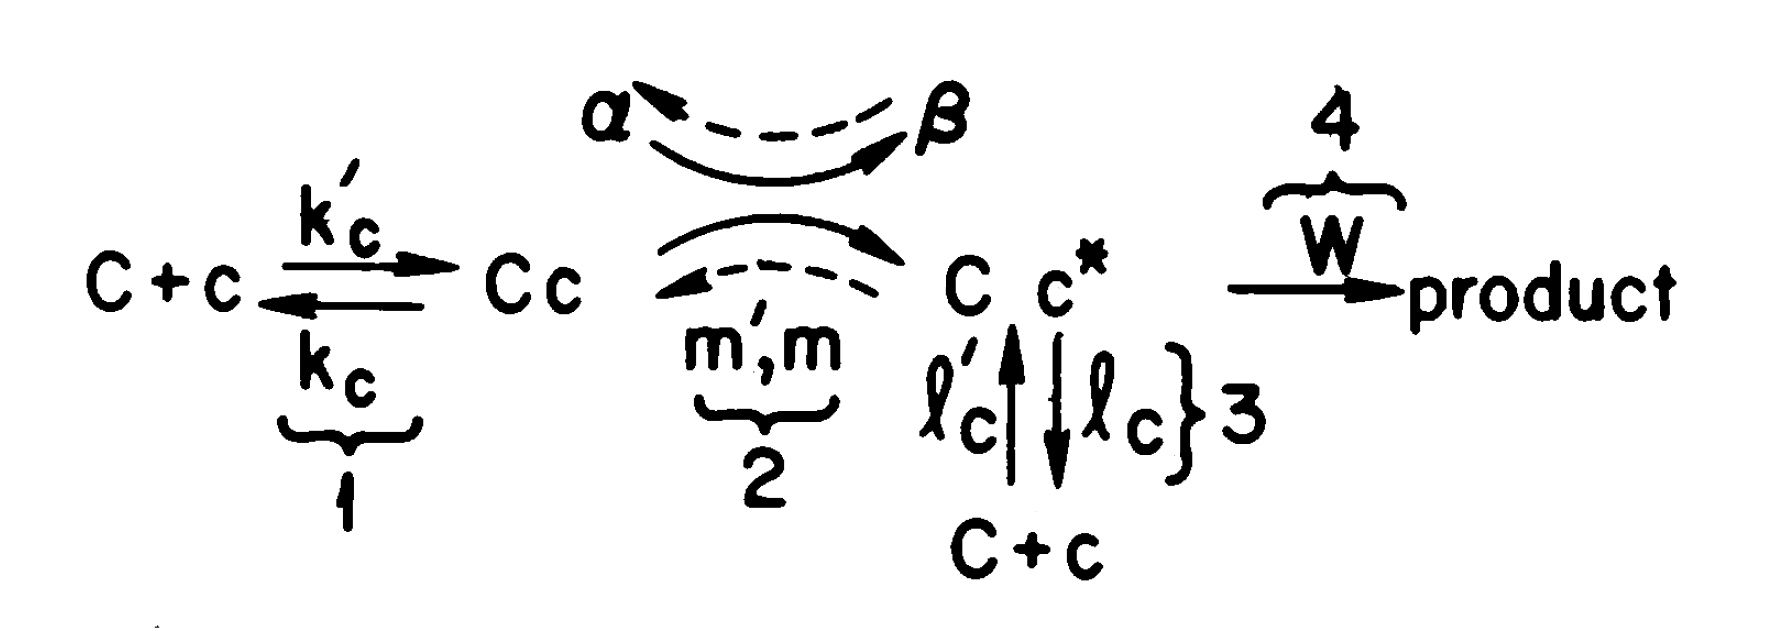
\includegraphics[width=\textwidth]{reaction8}
\end{frame}

\begin{frame}{Двухэтапная модель энергозависимой реакции} % TODO \only<...> or somethning

Если $ m $ и $ l'_C $ малы:

\begin{align*}
    C + c \overunderset{k'_C}{k_C}{\rightleftharpoons} Cc \overset{m'}{\rightarrow} \quad & Cc^* & \overset{W}\to \text{product} \\
    & \downarrow l_C & \\
    & C+c &
\end{align*}

\[ \frac{m'}{m} \gtrsim \left( \frac{1}{f_0} \right) \left( \frac{m'}{m} \right)_{equilib} \]

\end{frame}

\begin{frame}{Коррекция как реакция Михаэлиса}
	\begin{align*}
		C + c \rightleftharpoons Cc \rightarrow \quad & Cc^* & \overset{W}\to \text{product} \\
		& \downarrow & \\
		& C+c &
	\end{align*}

	
	\[ C + c \rightleftharpoons Cc \overset{W(t)}\to \text{product} \]
	
	\[ p_{incorporation} \approx \int_{0}^{\infty} e^{-k_C t} W(t) dt \]
\end{frame}

\begin{frame}{Пример: синтез белка }
\centering 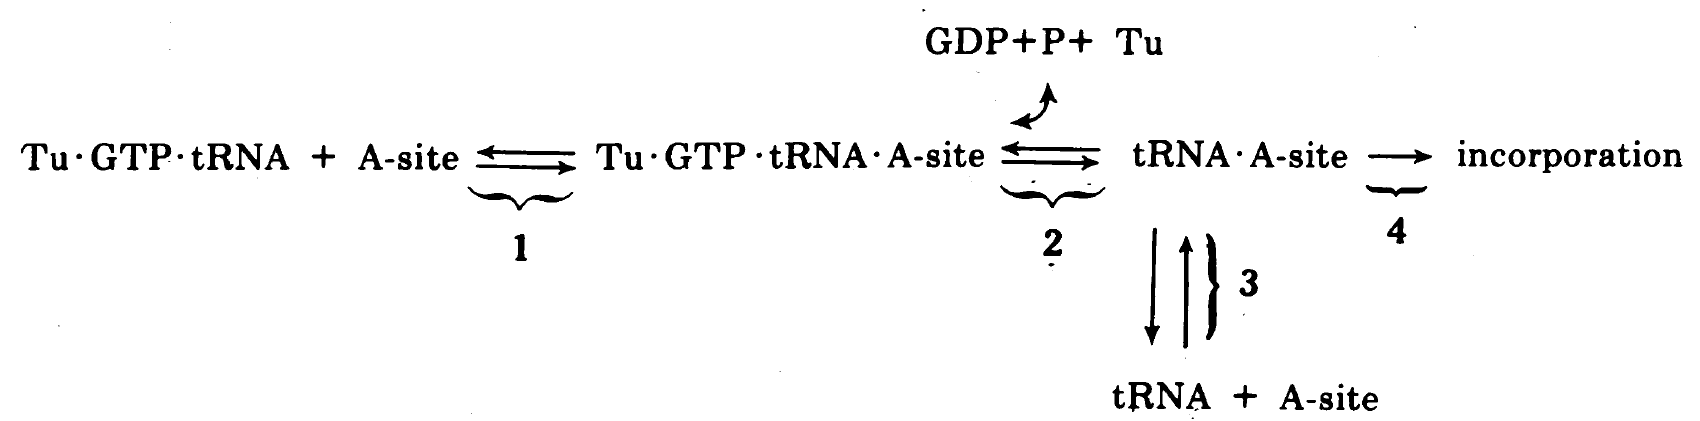
\includegraphics[width=\textwidth]{reaction_rna2protein}

\end{frame}

\begin{frame}{Пример: заряжаем тРНК}
Первый этап:

\centering 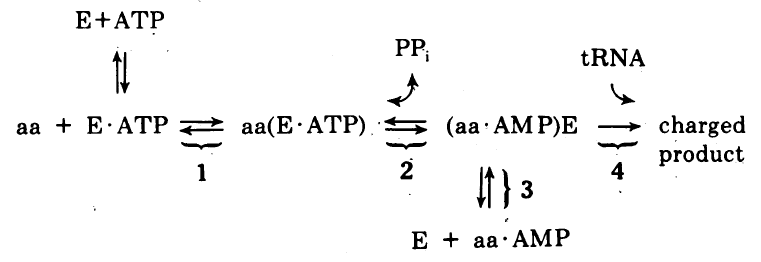
\includegraphics[width=.7\textwidth]{reaction_trna}

\flushleft (Вспомним)

\centering 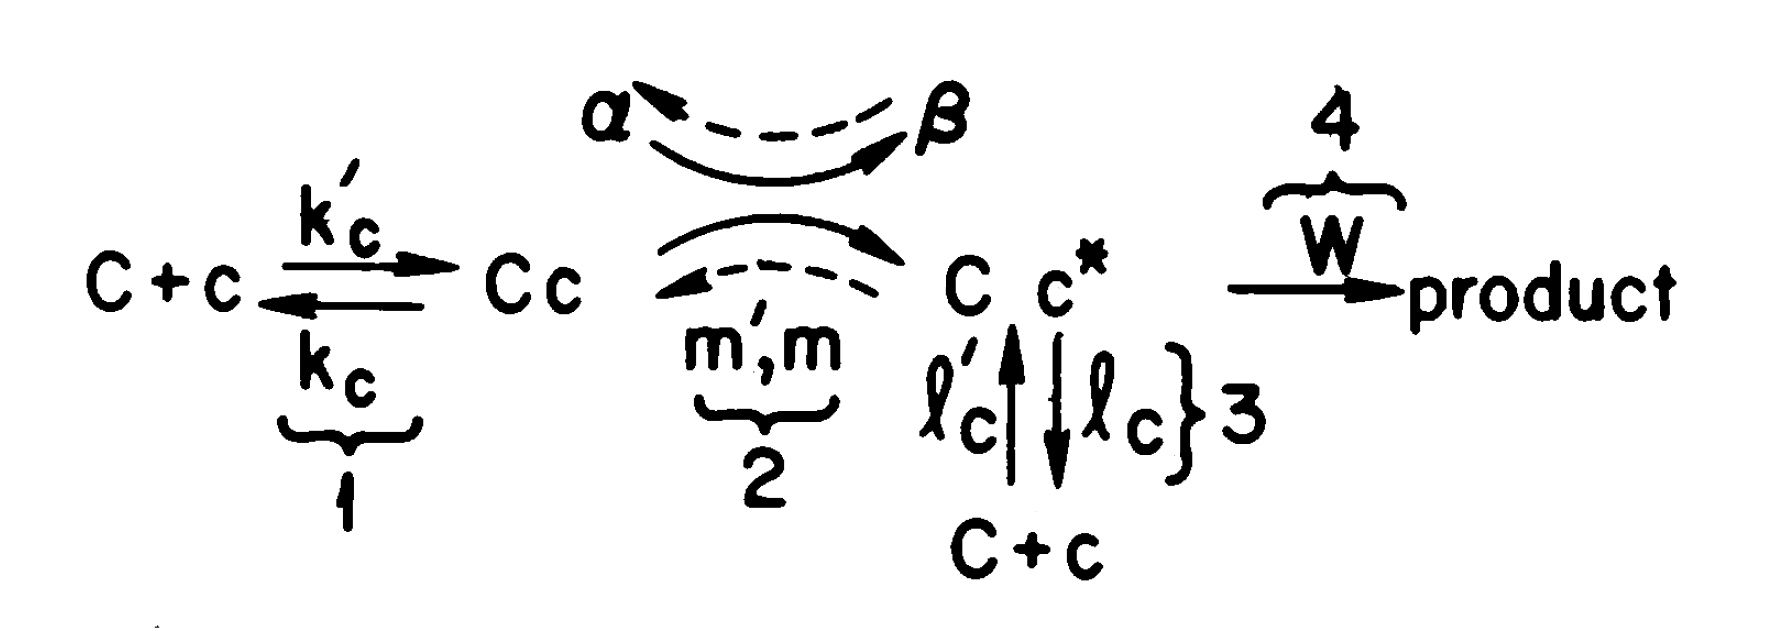
\includegraphics[width=.4\textwidth]{reaction8}

\end{frame}

\begin{frame}{Пример: репликация ДНК}
    \centering 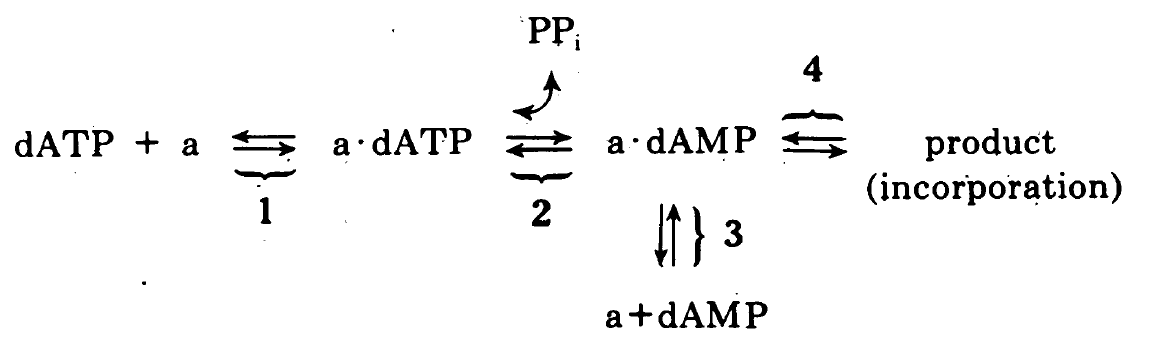
\includegraphics[width=.7\textwidth]{reaction_dna}

\end{frame}

\begin{frame}{Комментарии к презентации Даны}

Распределение Пуассона характеризуется тем, что Фано-Фактор равен 1: $ \sigma^2 = \mu \Rightarrow \frac{\sigma^2}{\mu} = 1 $

По сравнению с затратами на транскрипцию и трансляцию, это

Большой шум снижает выгоды большого динамического диапазона.
Они присутствуют одновременно и увеличиваются одновременно.

Максимизация mutual information: <<мы не знаем реальное значение $c$, давайте максимизируем матрицу mutual info>>.
Чем более сложное вещество, тем более модель похожа на наличие пруфридинга.

Предлагаются гипотезы о том, в каких организмах искать пруфридинг (мет).

\end{frame}

\end{document}
